\section{Конструкторская часть}

В данном разделе будут рассмотрены конкретные алгоритмы, которые были применены для обработки изображений, а также, будут описаны структуры данных, используемые в данной работе.

\subsection{Точечные фильтры}
\subsubsection{Нетагив}

Для применения этого фильтра все составляющие цвета каждого пискселя (R, G и B) нужно инвертировать -- вычесть текущее значение из 255 (так как максимальное значение -- 256).

\subsubsection{Преобразование к оттенкам серого}

Заключается в получении яркости каждой точки по формуле $Y = 0.3 * R + 0.59 * G + 0.11 * B$ и последующем копировании полученного значения во все три канала (R, G и B).

\subsection{Матрица свёртки}
Матрица свёртки -- это матрица коэффициентов, которая «умножается» на значение пикселей изображения для получения требуемого результата \cite{convolition}. 

Алгоритм применения следующий: начиная с верхнего левого пикселя, выделяется ядро размером матрицы свертки (рис. \ref{fig:spire11}); проводится перемножение между элементами матрицы свертки и выделенного ядра, для примера, показанного на рисунке \ref{fig:spire11}, результат будет следующим: $6\cdot0+6\cdot1+1\cdot0+3\cdot1+7\cdot2+5\cdot1+2\cdot0+3\cdot1+1\cdot0=31$. Далее вычисляется коэффициент нормирования, суммируя компоненты матрицы свёртки. Для примера это значение будет равно $0+1+0+1+2+1+0+1+0=6$; результат перемножения матриц делится на коэффициент нормирования: $\frac{31}{6}=5.167$; полученное значение присваевается центральному компоненту ядра. Весь цикл повторяется для каждого пикселя изображения.

\begin{figure}[hbtp]
	\centering
	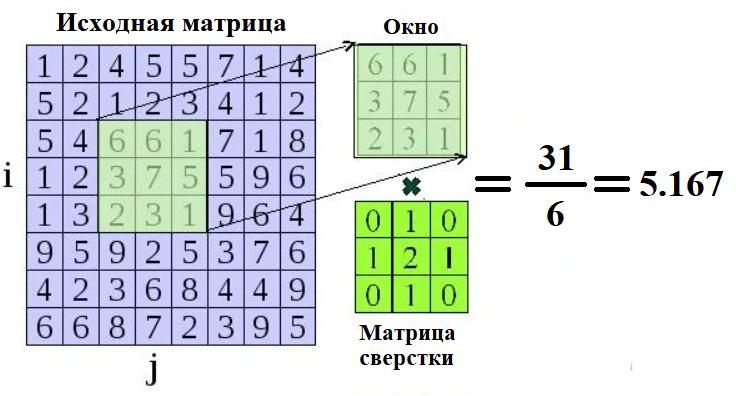
\includegraphics[width=\textwidth]{img/image5.png}
	\caption{\label{fig:spire11} Применение матрицы сверстки}
\end{figure}

\subsection{Фильтр размытия}

Наиболее часто используемым фильтром, основанным на матрице свёртки, является фильтр размытия. Фильтр меняет каждую точку выбранного ядра, делая её значение равным значению всех точек в определённом радиусе от рассматриваемой точки. Значение этого радиуса (размер матрицы) можно изменить.

Обычно матрица заполняется по нормальному (Гауссовому) закону. 

\subsubsection{Нормальное распределение}
Главная особенность нормального закона распределения заключается в том, что он является предельным законом для других законов распределения. Нормальное распределение случайной величины -- одно из непрерывных распределений, имеющее основополагающую роль в математической статистике \cite{normDistr}.

В нормальном распределении, чем ближе к центральной точке, тем больше значение, а чем дальше от центра, тем меньше значение (рисунок \ref{fig:spire13}).
При вычислении среднего значения нам нужно только использовать «центральную точку» в качестве начала координат и присвоить веса другим точкам в соответствии с их положениями на нормальной кривой, чтобы получить средневзвешенное значение. Нормальное распределение, очевидно, является желательной моделью распределения веса.

\begin{figure}[hbtp]
	\centering
	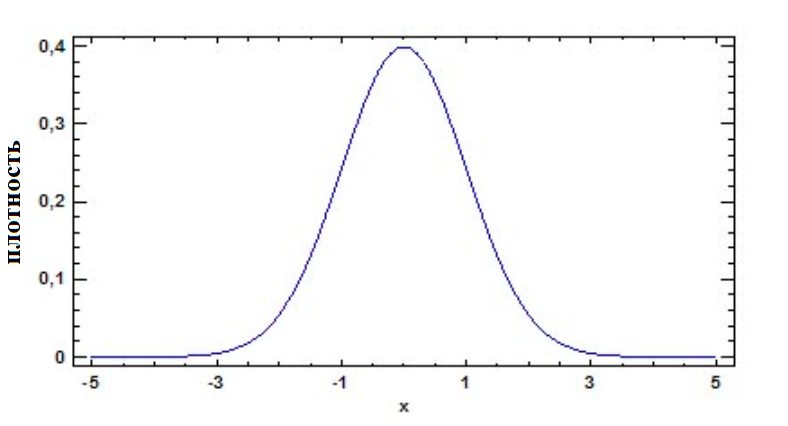
\includegraphics[width=0.8\textwidth]{img/image6.png}
	\caption{\label{fig:spire13} Нормальное распределение}
\end{figure}

\subsubsection{Функция Гаусса}

Функция плотности нормального распределения называется «функцией Гаусса» \cite{gauss}. Его одномерная форма (\ref{for:gauss1}).

\begin{equation}
	\label{for:gauss1}
	f(x) = \frac{1}{\sigma\sqrt{2\pi}} \cdot \exp^{-(x-\mu)^2/2\sigma^2}
\end{equation}
где: \(\mu\) — среднее значение \(x\), \(\sigma\) — дисперсия\footnote{Дисперсия — это величина, показывающая, как именно и насколько сильно разбросаны значения.}  \(x\). Поскольку при вычислении среднего значения центром является начало координат, поэтому \(\mu\) равно 0 (\ref{for:gauss2}).

\begin{equation}
	\label{for:gauss2}
	f(x) = \frac{1}{\sigma\sqrt{2\pi}} \cdot \exp^{-x^2/2\sigma^2}
\end{equation}
В соответствии с одномерной функцией Гаусса, двумерная функция Гаусса может быть получена как (\ref{for:gauss3}).
\begin{equation}
	\label{for:gauss3}
	G(x,y) = \frac{1}{2\pi\sigma^2} \cdot \exp^{-(x^2+y^2)/2\sigma^2}
\end{equation}
С помощью этой функции можно рассчитать вес каждой точки.

В таблице \ref{gaussTable} приведена матрица размытия 5x5, заполненная по закону Гауссовского распределения.

\begin{table}[hbtp]
	\centering
	\begin{tabular}{|l|l|l|l|l|}
		\hline
		0.000789 & 0.006581 & 0.013347 & 0.006581 & 0.000789 \\ \hline
		0.006581 & 0.054901 & 0.111345 & 0.054901 & 0.006581 \\ \hline
		0.013347 & 0.111345 & 0.225821 & 0.111345 & 0.000789 \\ \hline
		0.006581 & 0.054901 & 0.111345 & 0.054901 & 0.006581 \\ \hline
		0.000789 & 0.006581 & 0.013347 & 0.006581 & 0.000789 \\ \hline
	\end{tabular}
	\caption{\label{gaussTable} Матрица размытия 5x5, заполненная по закону Гауссовского распределения}
\end{table}

Матрица уже нормированна, поэтому, ее определитель равен 1. От размера матрицы зависит сила размытия.

\subsection{Медианный  фильтр}

Медианный фильтр является примером нелинейной фильтрации, обычно используется для уменьшения шума или «сглаживания» изображения.

Фильтр работает с матрицами различного размера, но в отличие от матрицы свёртки, размер матрицы влияет только на количество рассматриваемых пикселей.
Алгоритм медианного фильтра следующий: для текущего пикселя, пиксели, которые «попадают» в матрицу, сортируются, и выбирается средние значение из отсортированного массива. Это значение и является выходным для текущего пикселя.

На рисунке \ref{fig:spire15} представлена работа медианного фильтра для размера ядра равного трём.

\begin{figure}[hbtp]
	\centering
	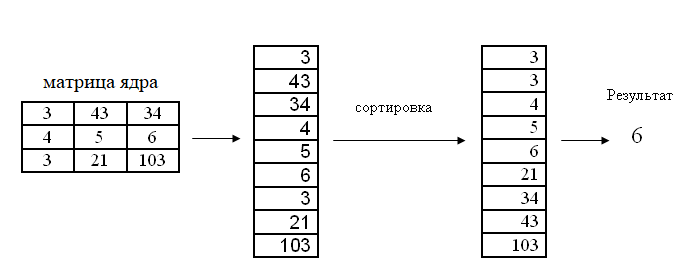
\includegraphics[width=\textwidth]{img/image7.png}
	\caption{\label{fig:spire15} Работа медианного фильтра}
\end{figure}

\subsection{Проблема матричных фильтров}

Стоит упомянуть о граничных условиях (эта проблема актуальна для всех матричных фильтров). У верхнего левого пикселя не существует «соседа» с права от него, следовательно, нам не на что умножать коэффициент матрицы (рисунок \ref{fig:spire16}).

\begin{figure}[hbtp]
	\centering
	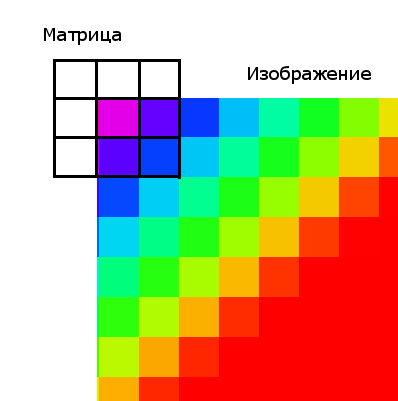
\includegraphics[width=0.6\textwidth]{img/image8.png}
	\caption{\label{fig:spire16} Проблема применения матричных фильтров}
\end{figure}

Существует 2 решения этой проблемы.


Первое решение заключается в применении фильтра, только к «окну» изображения (рисунок \ref{fig:spire17}), которое имеет координаты левого верхнего угла \newline $(kernelSize / 2, kernelSize / 2)$, а для правого нижнего \newline $(width — kernelSize / 2, height — kernelSize / 2)$, где kernelSize – размер матрицы, а width и height – размеры изображения.

\begin{figure}[hbtp]
	\centering
	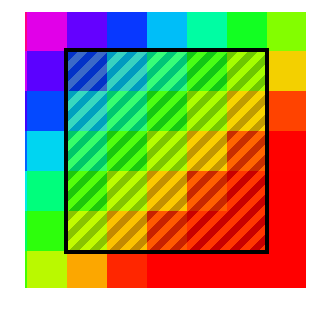
\includegraphics[width=0.6\textwidth]{img/image9.png}
	\caption{\label{fig:spire17} Применение фильтра, только к «окну» изображения}
\end{figure}

Второй метод (рисунок \ref{fig:spire18}) требует создания промежуточного изображения. Идея в том, чтобы создавать временное изображение с размерами $(width + 2 * kernelSize / 2, height + 2 * kernelSize / 2)$. В центр изображения копируется входная картинка, а края заполняются крайними пикселями изображения. Размытие применяется к промежуточному буферу, а потом из него извлекается результат.

\begin{figure}[hbtp]
	\centering
	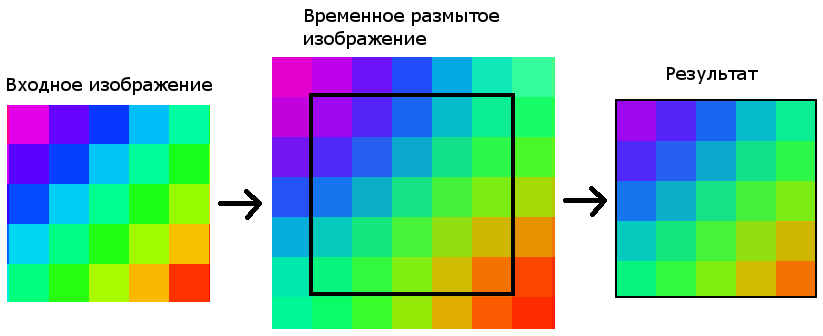
\includegraphics[width=\textwidth]{img/image10.png}
	\caption{\label{fig:spire18} Дополнение}
\end{figure}

Данный метод не имеет недостатков в качестве, но необходимо производить лишние вычисления.	

\subsection{Выбор используемых типов и структур данных}

Для разрабатываемого ПО необходимо реализовать следующие типы и
структуры данных.

\begin{enumerate}[leftmargin=1.6\parindent]
	\item[1.] Структура BITMAPFILEHEADER -- заголовок файла BMP:
	\begin{enumerate}[leftmargin=1.6\parindent]
		\item[---] $unsigned\ int\ bfType$ -- тип файла;
		\item[---] $unsigned\ long\ bfSize$ -- размер в байтах;
		\item[---] $unsigned\ int\ bfReserved1$ и $bfReserved2$ -- зарезервинованные (нули);
		\item[---] $unsigned\ long\ bfOffBits$ -- смещение.
	\end{enumerate} 
	\item[2.] Структура BITMAPINFOHEADER -- содержание файла:
	\begin{enumerate}[leftmargin=1.6\parindent]
		\item[---] $unsigned\ int\ biSize$ -- тип размер структуры;
		\item[---] $size\_t\ biWidth$ и $biHeight$ -- ширина и высота картинки соответственно;
		\item[---] $unsigned\ short\ biPlanes$ -- количество плоскостей;
		\item[---] $unsigned\ short\ biBitCount$ -- количество бит на пиксель;
		\item[---] $unsigned\ int\ biCompression$ -- тип сжатия;
		\item[---] $unsigned\ int\ biSizeImage$ -- размер картинки в байтах;
		\item[---] $int\ biXPelsPerMeter$ и $biYPelsPerMeter$ -- горизонтальное и вертикальное разрешение соответственно;
		\item[---] $unsigned\ int\ biClrUsed$ -- количество исп. цветов;
		\item[---] $unsigned\ int\ biClrImportant$ -- количество важных цветов.
	\end{enumerate} 
	\item[3.] Структура RGBQUAD -- пиксель в формате RGB:
	\begin{enumerate}[leftmargin=1.6\parindent]
		\item[---] $double\ rgbBlue -- синий цвет$;
		\item[---] $double\ rgbGreen -- зеленый цвет$;
		\item[---] $double\ rgbRed -- красный цвет$;
		\item[---] $double\ rgbReserved -- зарезервировано$.
	\end{enumerate} 
	\item[4.] Cnhernehf PIX -- пиксель:
	\begin{enumerate}[leftmargin=1.6\parindent]
		\item[---] $double\ value$ -- значение пикселя;
		\item[---] $RGBQUAD\ rgb$ -- его значение в RGB.
	\end{enumerate} 
\end{enumerate} 

\subsection*{Выводы}

В данном разделе были рассмотрены конкретные алгоритмы, которые применялись для обработки изображений, была рассмотрена проблема, которая встречается при работе с матричными фильтрами, и пути ее решения. Кроме того, были описаны выбранные структуры данных.


\pagebreak